\documentclass{scrartcl}

\usepackage{syntax} % for BNFs
\usepackage{graphicx} % for the logos
\usepackage{calc} % for header width computation
\usepackage{multirow}
\usepackage{amssymb} % for triangleq

\usepackage{listings}
\lstset{mathescape}

\usepackage{array}   % for \newcolumntype macro
\newcolumntype{L}{>{$}l<{$}} % math-mode version of 'l' column type
\newcolumntype{R}{>{$}r<{$}} % math-mode version of 'r' column type
\newcolumntype{C}{>{$}c<{$}} % math-mode version of 'c' column type

\newcommand*{\getAndInc}[1]{\arabic{#1}\stepcounter{#1}}

\newcommand*{\optional}[1]{#1\mathord{?}}

\newcommand*\makeHeader[1]{%
  { 
    \setlength{\parskip}{0pt}
    \hrule height 1pt
    \vspace{.2cm}
    \hspace{-.4cm}
    \begin{minipage}[t][20mm][b]{20mm}
    {
      
\includegraphics[height=20mm]{logouni.pdf}
    }
    \end{minipage}
    \begin{minipage}[t][20mm][c]{\textwidth-42mm}
    \begin{center} \raisebox{-.7cm}{\Huge{\textbf{#1}}} \end{center}
    \end{minipage}
    \begin{minipage}[t][20mm][b]{20mm}
    {
      \raisebox{-7mm}{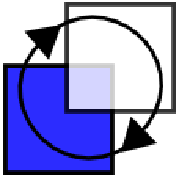
\includegraphics[height=20mm]{logoreact.pdf}}
    }
    \end{minipage}
    \par
    \vspace{.2cm}
    \hrule height 1pt
  }
}

\begin{document}    
\setlength{\grammarindent}{8em} % increase separation between LHS/RHS 

    
  \makeHeader{Lola Syntax}
  
  \section{Abbreviations}

  \begin{itemize}
    \item square brackets denote comma separated non-empty lists of non-terminals, i.e.,
    \begin{lstlisting}
      [A] $\triangleq$ A (`,' A)*  
    \end{lstlisting}
    \item The unary postfix $\mathord{?}$-operator denotes an optional category, i.e.,
    \begin{lstlisting}
      A? $\triangleq$ $\epsilon$ | A
    \end{lstlisting}
    \item The unary postfix $+$-operator denotes the non-empty repetition, i.e.,
    \begin{lstlisting}
      A+ $\triangleq$ A A*
    \end{lstlisting}
  \end{itemize}
  
  
  
  \section{Instance Specification}
  \begin{grammar}
    <EffectiveConstant> ::= <Literal> | <Parameter>
  
    <StreamInstance> ::= <Ident> (`(' [<EffectiveConstant>] `)')?
  \end{grammar}
  
  \section{Expressions}
  
  \begin{grammar}
    <Expression> ::= %
      <UnaryOperator> <Expression>
      \alt <Expression> <BinaryOperator> <Expression>
      \alt <FunctionName> `(' [<Expression>] `)'
      \alt <Expression> `?' <Expression>
      \alt <StreamInstance> `[' (<TimeOffset> | <EffectiveConstant>) `]'
      \alt <StreamInstance>` [' <Duration> `,' <WindowOperator> `]'
      \alt `if' <Expression> `then' <Expression> `else' <Expression>
      \alt <Literal>
      \alt <Ident>
      \alt <Ident>.<Ident>
      \alt `(' <Expression> `)'
      \alt `(' (<Expression> (`,' <Expression>)*)? `)'
  \end{grammar}
    
    
  \section{Declarations and Statements}
  
  \begin{grammar}
  
  <TemplateSpec> ::= \ \\
      `{' \\
        (`invoke:' <Expression> ((`if' | `unless') Expr)?)? \\
        (`extend:' <Expression>? (`@' <Frequency>)?)? \\
        (`terminate:' <Expression>)? \\
      `}'
      
  <IncludeStatement> ::= `include' <StringLiteral>
  
  <TypeDeclaration> ::= `Type' <Ident> `{' [<Type> <Ident>] `}'
  
  <ConstantStream> ::= `constant' <Type> <Ident> := <Literal>
  
  <InputStream> ::= `input' <Type> [<Ident> (`<'[<Type> <Ident>]`>')?]
  
  <OutputStream> ::= `output' <Type> <Ident> (`<'[<Type> <Ident>]`>')? <TemplateSpec>? `:=' <Expression>
  
  <Trigger> ::= `trigger' <Ident>? <Expression> <StringLiteral>?
  
  <LanguageSpec> ::= `//!' (`ClassicLola' | `Lola2.0' | `RTLola')
  
  <LolaSpecification> ::= <LanguageSpec>? (<IncludeStatement> | <TypeDeclaration> | <ConstantStream> | <InputStream> | <OutputStream> | <Trigger>)+
    
  \end{grammar}

  \section{Operators}
  
  \newcounter{prec}
  \setcounter{prec}{1}
  
  \begin{tabular}{c | l | l | C} 
  Precedence & Name & \mbox{Associativity} & \mbox{Example} \\ \hline
  \multirow{3}{*}{\getAndInc{prec}} & Field Access          & left  & a.b         \\ \cline{2-4}
                                    & Stream Access         & -     & s[1]        \\ \cline{2-4}
                                    & Functions             & -     & \sin(3)     \\ \hline
  \getAndInc{prec}                  & Default Operator      & -     & s[1] ? 3    \\ \hline
  \getAndInc{prec}                  & Unary Operators       & -     & +, -, !     \\ \hline
  \getAndInc{prec}                  & Exponentiation        & right & **          \\ \hline
  \getAndInc{prec}                  & Multiplication        & left  & *, /, \%    \\ \hline
  \getAndInc{prec}                  & Addition              & left  & +, -        \\ \hline
  \getAndInc{prec}                  & Comparison            & -     & =, !=, >    \\ \hline
  \getAndInc{prec}                  & Logic Conjunction     & left  & \&, \land   \\ \hline
  \getAndInc{prec}                  & Logic Disjunction     & left  & |, \lor     \\ \hline
  \getAndInc{prec}                  & If-Then-Else          & -     & \mbox{if/then/else} 

    
  \end{tabular}



\end{document}